\autsubsection{ESA's Deep Space Communication Network}{Gustavo Feijóo Carrillo}

%*The International Telecommunications Union (ITU) defines Deep Space (DS) to start at a distance of 2 million km from the Earth's surface. Allocated frequency bands for DS operation according to ITU are:

%>S-Band: 2110-2120 MHz uplink, 2290-2300MHz downlink.
%>X-Band: 7145-7190 MHz uplink, 8400-8450MHz downlink.
%>Ka-Band: 34.2-34.7 GHz uplink, 31.8-32.3GHz downlink.

%ESA is today autonomously flying several interplanetary missions like Rosetta and MarsExpress. The capability of supporting present and future DS missions is the consequence of a farsighted decision, taken in 1996, to expand the network of 15m tracking antennas into the DS domain. The ambitious plan of deploying three 35m DS antennas over the world, ensuring around the clock coverage to all interplanetary missions, has been recently completed. These three DS antennas, DSA1 located in New Norcia (Australia), DSA2 in Cebreros (Spain) and DSA3 in Malargue (Argentina), are in operation since 2002, 2005 and 2013 respectively.


%*Technical facilities comprise X-band transmission and X- and Ka-Band reception, plus facilities for tracking, telemetry, telecommand and radiometric measurements
    
%*The station is also equipped with Delta DOR (Delta Differential One-Way Ranging) capability, a new technology enabling highly precise spacecraft location and tracking.
    
\begin{figure}[htb]
	\centering
	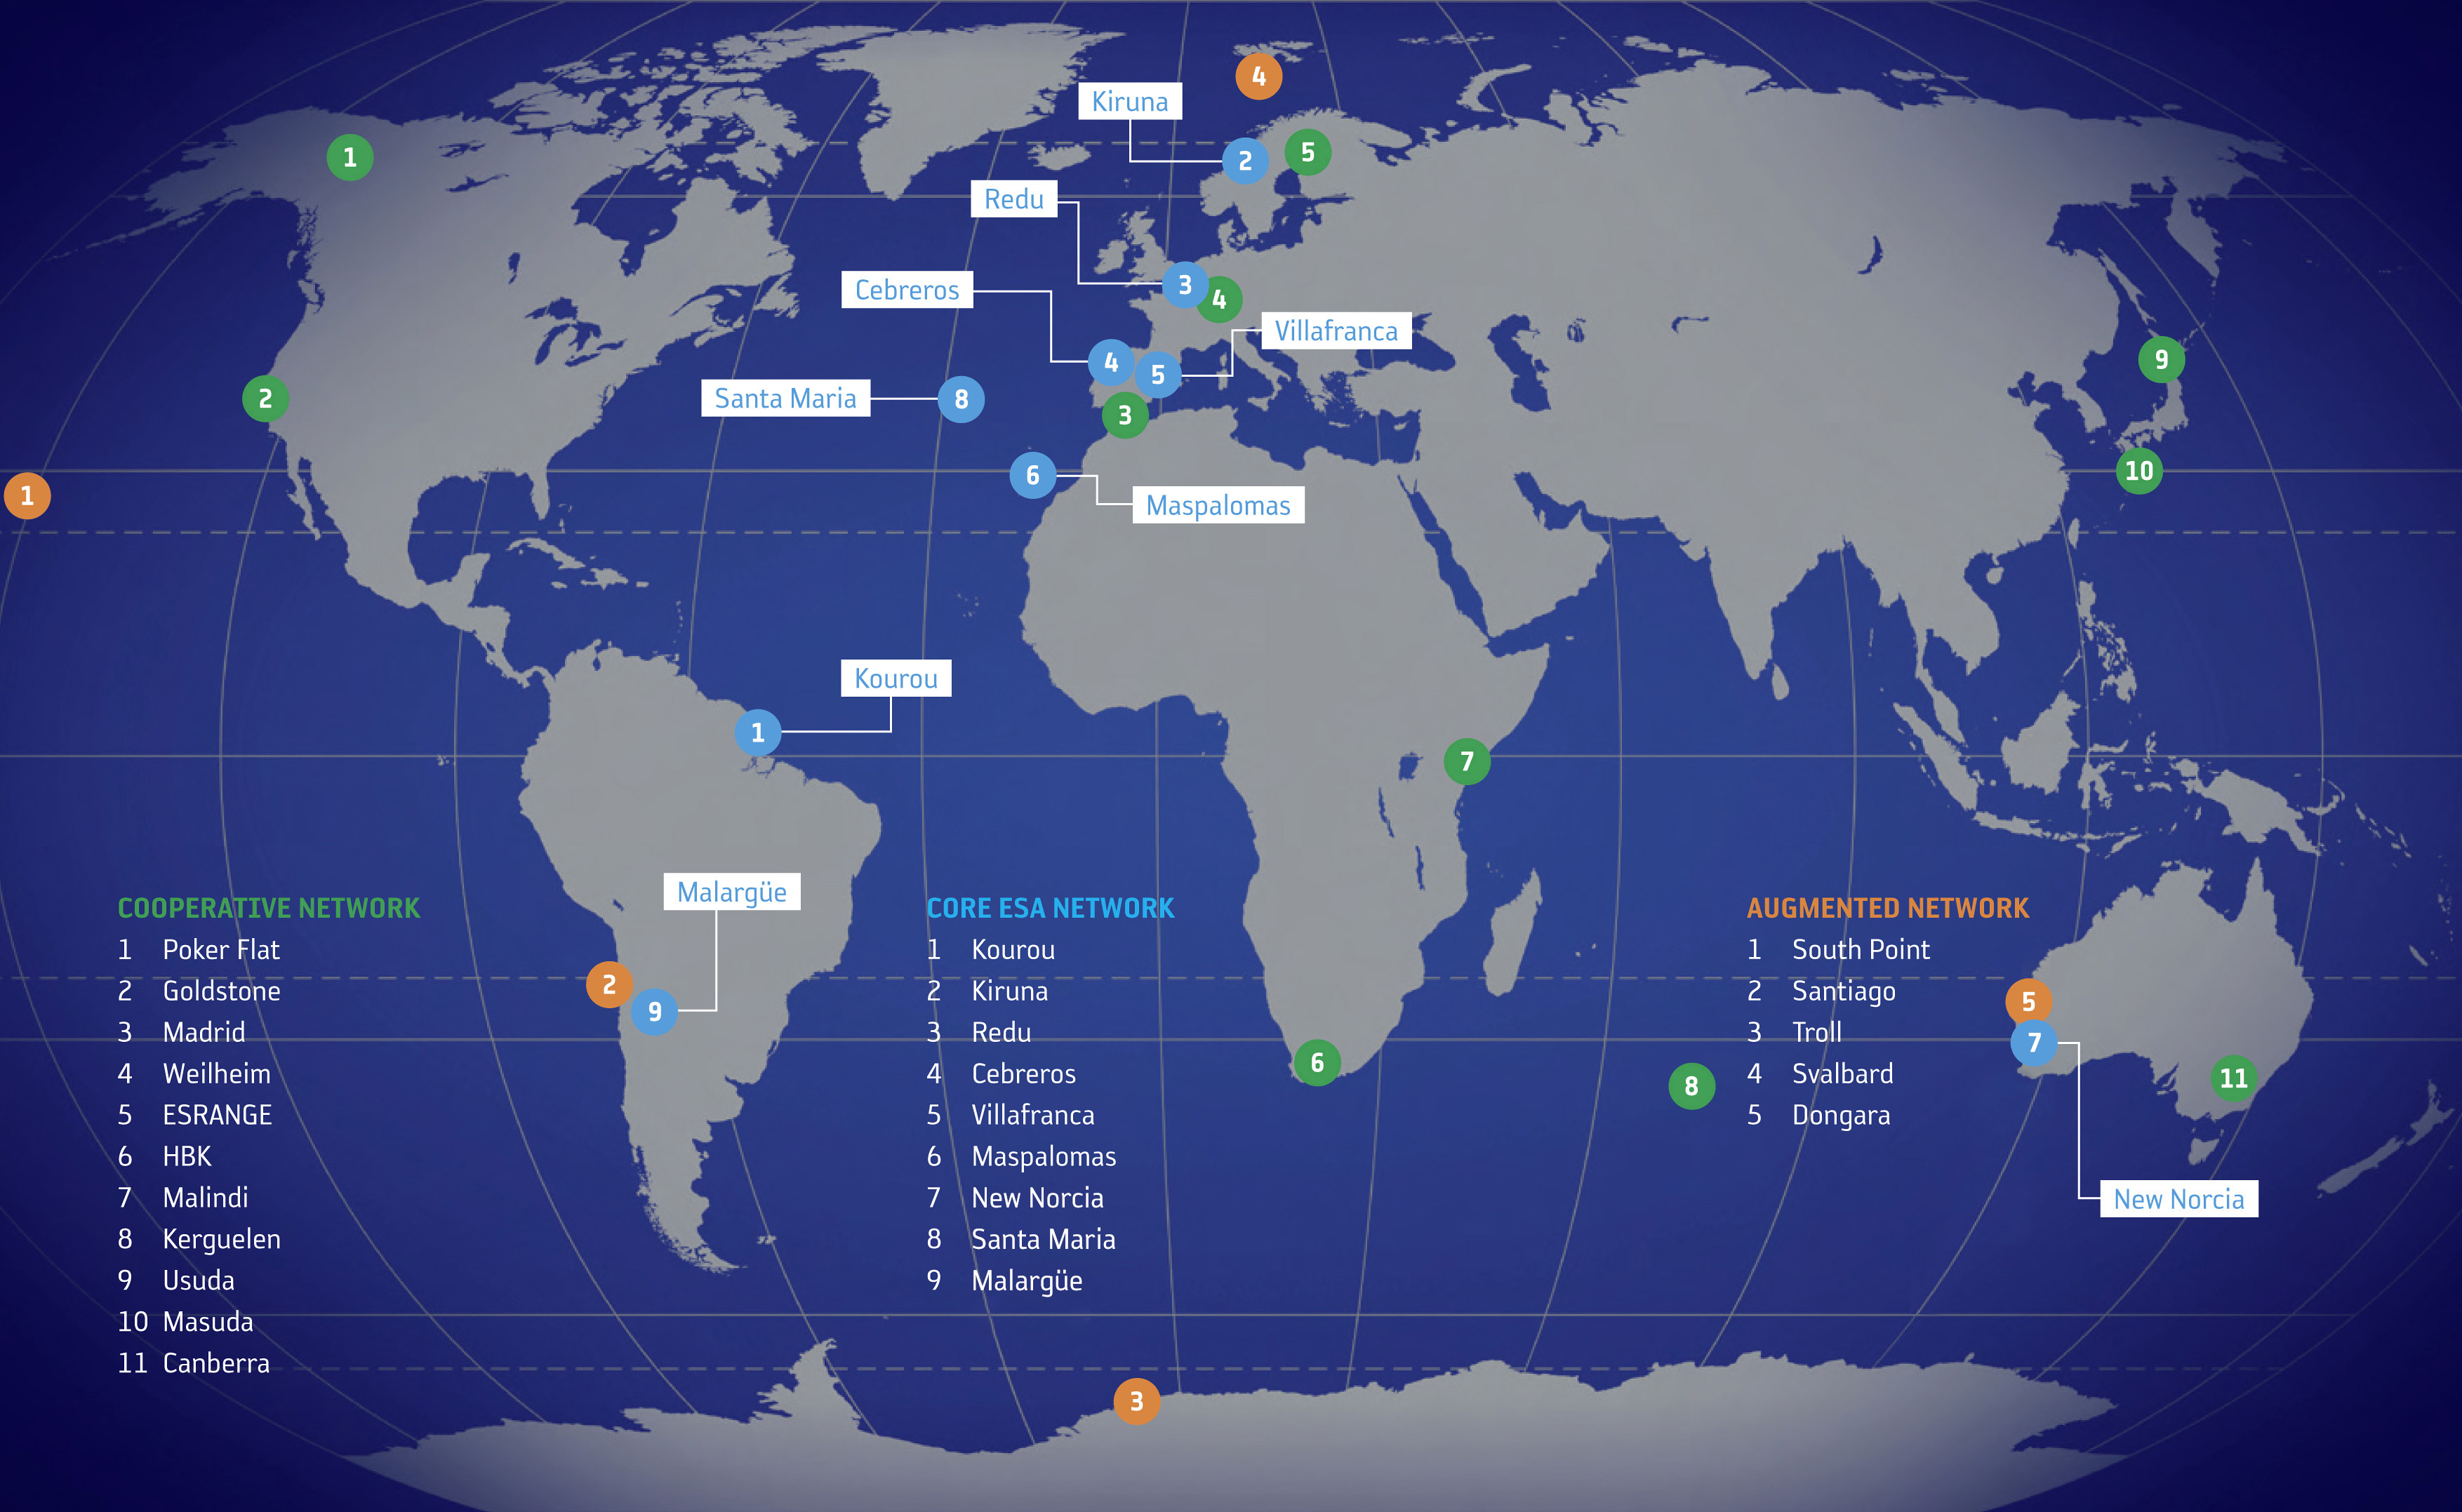
\includegraphics[width=\textwidth]{figures/comms/ESTRACK-map}
	\caption{Map of ESA's ESTRACK network, allowing for deep space communication and tracking of the spacecraft.}
	\label{fig:ESTRACK-map}
\end{figure}